\documentclass[conference]{IEEEtran}
\usepackage{cite}
\usepackage{amsmath,amssymb,amsfonts}
\usepackage{algorithmic}
\usepackage{graphicx}
\usepackage{textcomp}
\usepackage{xcolor}
\usepackage{array}
\usepackage{ragged2e}
\usepackage{multirow} % For multirows in tables
\usepackage{float} % Appending the [H] option forces the placement of a figure in the place it's in the code
\usepackage[numbers]{natbib} % For integration with bibliography commands

% BEGIN The following is for typesetting Verilog
\usepackage{xcolor}
\usepackage{listings}
\definecolor{vgreen}{RGB}{104,180,104}
\definecolor{vblue}{RGB}{49,49,255}
\definecolor{vorange}{RGB}{255,143,102}
\lstdefinestyle{verilog-style}{
    language=Verilog,
    basicstyle=\small\ttfamily,
    keywordstyle=\color{vblue},
    identifierstyle=\color{black},
    commentstyle=\color{vgreen},
    numbers=left,
    numberstyle=\tiny\color{black},
    numbersep=3pt,
    tabsize=4,
    moredelim=*[s][\colorIndex]{[}{]},
    literate=*{:}{:}1
}
\makeatletter
\newcommand*\@lbracket{[}
\newcommand*\@rbracket{]}
\newcommand*\@colon{:}
\newcommand*\colorIndex{%
    \edef\@temp{\the\lst@token}%
    \ifx\@temp\@lbracket \color{black}%
    \else\ifx\@temp\@rbracket \color{black}%
    \else\ifx\@temp\@colon \color{black}%
    \else \color{vorange}%
    \fi\fi\fi
}
\makeatother
% END

\begin{document}

\title{Lab 3 Report --- Block RAM\\
\Large{Computer Design Laboratory ECE 3710}\\
\Large{Fall 2021}\\
\Large{The University of Utah}}

\author{\IEEEauthorblockN{Jacob Peterson}
\IEEEauthorblockA{\textit{Computer Engineering 2022}\\
\textit{University of Utah}\\
Salt Lake City, UT}
\and
\IEEEauthorblockN{Brady Hartog}
\IEEEauthorblockA{\textit{Computer Engineering 2022}\\
\textit{University of Utah}\\
Salt Lake City, UT}
\and
\IEEEauthorblockN{Isabella Gilman}
\IEEEauthorblockA{\textit{Computer Engineering 2023}\\
\textit{University of Utah}\\
Salt Lake City, UT}
\and
\IEEEauthorblockN{Nate Hansen}
\IEEEauthorblockA{\textit{Computer Engineering 2023}\\
\textit{University of Utah}\\
Salt Lake City, UT}
}

\maketitle

\begin{abstract}
This paper details the design and synthesis of a simple Verilog module for a 1024-byte instantiation of Block RAM on a Cyclone V FPGA. This module will be used as a component for a model CPU that resembles the CR16. As such, we ensured that this BRAM module would be dual-port and allow for simultaneous read and write operations. We demonstrated the correct read-write functionality of our BRAM in multiple ways. We used a Verilog testbench to demonstrate correct operation of the virtual hardware, and we built a simple FSM to demonstrate the correct behavior of the memory in hardware. We are prepared to expand the capacity of this module should 1024 bytes prove insufficient for our purposes. This preliminary demonstration is meant only to show correct operation of the module. Adjustments to parameterization or behavior may be made at a later date as we better understand what we need the CPU to accomplish.
\end{abstract}

\section{Introduction}
The Cyclone V offers many options for data storage. We need our CR16 to be able to pre-load files to begin program execution when we synthesize and flash the FPGA. From the beginning we have been designing CPU datapath elements for 16-bit words, so our memory will store data in that width. We chose to use two M10K memory blocks for the purposes of this lab. The section ``BRAM Hardware Details on Cyclone V" justifies this decision.

Intel Quartus Prime provides various templates of code that will synthesize as Block RAM on the FPGA. We utilized one of these templates to code our RTL design and implement data preloading from a file. We added some customization to the template to make the module easier to use when we integrate it with the CR16. We tested the RTL in simulation using a testbench, and we tested its capability on the board using a simple FSM module with hard-coded reads/writes. Our tests are designed to cover all the possible behaviors of a true dual-port RAM--two simultaneous reads, two simultaneous writes, and a simultaneous read/write. Our module is demonstrably operable in simulation and on the FPGA.

Finally, we review the synthesis reports provided by Quartus Prime to analyze the M10K's resource use and gather information that will help us to make decisions about future trade-offs with our design. This information will guide our design practice as we move on to the full integration of datapath elements into the completed CR16 CPU.

\section{BRAM Hardware Details on Cyclone V}
 We determined that the RAM block should have true dual-port capabilities to integrate seamlessly with the functionality of our CR16 CPU. True dual-port mode is only available on the Cyclone V FPGA using the M10K memory block. For the purposes of this lab, we will instantiate two units of 512x16-bit M10K memory. We will only use two units for testing purposes, but we have the option to include as many as 397 units based on FPGA capacity \cite{handbook}. It makes sense to use 16-bit words for a 16-bit PC. However, we have capability to expand the scheme to as many as 20 bits. This is good to keep in mind in the event that we need to augment instruction length to add capability to the CPU when we put it to work. The volume capabilities of each M10K unit are detailed in the table in Fig. \ref{figure:m10k_table}.

 \begin{figure}[h]
     \centering
     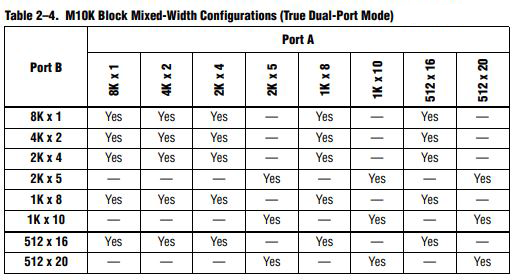
\includegraphics[scale=0.65]{resources/figures/bram_table_a.png}
     \caption{Table for width configurations of the M10K memory unit in true dual-port mode. \cite{handbook}}
     \label{figure:m10k_table}
 \end{figure}

 Based on the documentation, it is unclear where this memory block exists on the physical FPGA. We will be able to interpret its resource occupation from the synthesis reports after coding and synthesizing an RTL instance. Once we have that information, we can determine the possible trade-offs that come with expanding the memory capacity and adding future functional elements like an instruction decoder, program counter, and datapath combination. Many of these decisions will be made after the CR16 has been implemented and we have a more complete perspective.

 \begin{figure*}
     \centering
     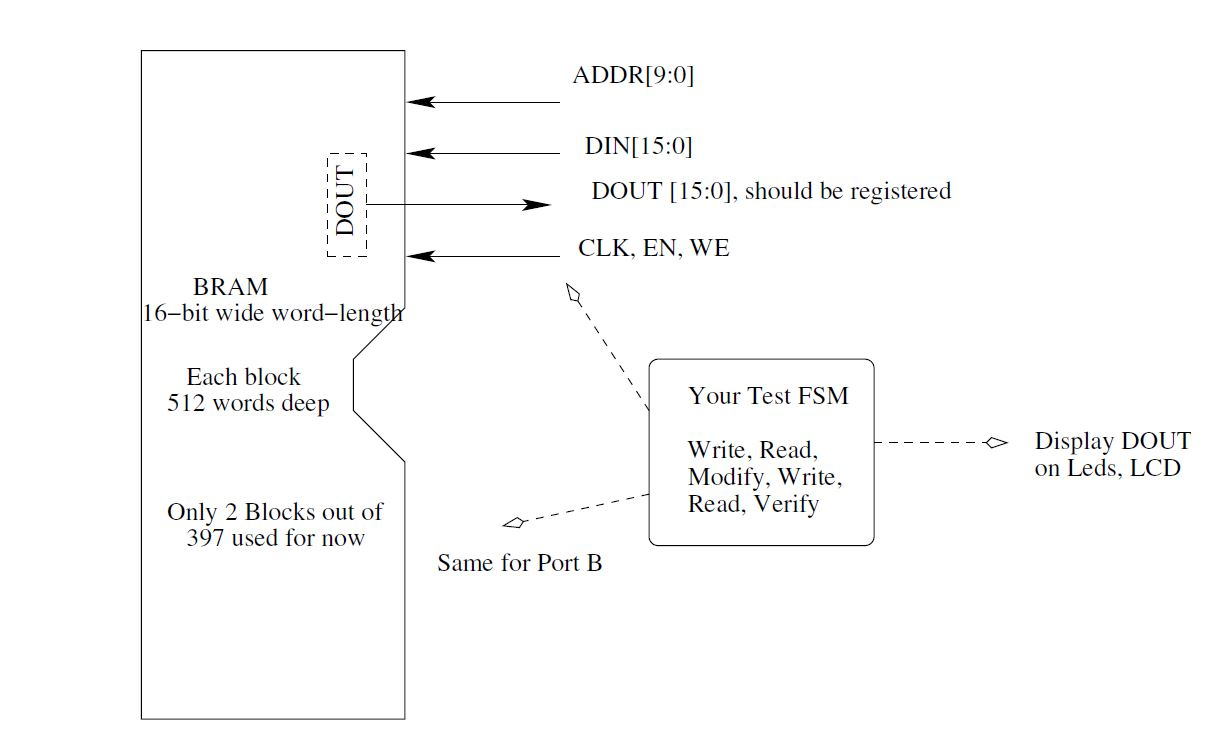
\includegraphics[scale=0.6]{resources/figures/block_diagram_bram.jpg}
     \caption{Block diagram for 2 units of 512x16-bit Block RAM with true dual-port capabilities.}
     \label{fig:block_diagram}
 \end{figure*}

For now, we will follow a general model as outlined by the block diagram in Fig. \ref{fig:block_diagram}.

\section{BRAM RTL}
The RTL for our BRAM module was adapted from a template generated by Quartus Prime. It supports simultaneous reading and writing via a dual-port interface with I/O data lines and address lines for each port. The module is completely parameterized allowing for a variable data width and address width. It also supports initializing the BRAM upon FPGA programming or flashing given a UTF-8-encoded initialization file via the \verb|readmemh| Verilog system task. This initialization file simply contains n-bit hex values on every line where each line corresponds to the data at a given memory address. Additionally, the parameter list allows address offsetting to be used so that a module instantiation with a BRAM initialization file can be pre-loaded at a specific address in BRAM. If no initialization file is given, then the entirety of BRAM is initialized to zeros.

The register array contained within the BRAM module consists of a 2-dimensional array where the first dimension is an unpacked array representing a word and the second dimension is a packed array containing the bits of a word. There are two \verb|always| blocks sensitive to the \verb|posedge| of the clock signal---one block for port A and one for port B. If the \verb|I_WRITE_ENABLE| signal on the given port is asserted, then the value from the data inputs are written to the register array at the given address and the output data is latched to its value from the previous clock cycle. If the \verb|I_WRITE_ENABLE| signal on the given port is reset, then the output data lines get the word contained in register array at the given address.

According to synthesis reports, the body of this BRAM module gets ``synthesized away'' upon compilation and synthesis within Quartus Prime. Since the BRAM already exists on the FPGA, there is no need to synthesize this module completely and utilize logic elements, but instead, connections are made between the BRAM on the FPGA and the \verb|input| and \verb|output wires| declared in a \verb|bram| module instantiation.

The signature and body of our BRAM module is shown in Figure \ref{figure:bram_module}.

\begin{figure*}
    \begin{lstlisting}[style={verilog-style}]
module bram
       #(parameter P_BRAM_INIT_FILE = "",
         parameter integer P_BRAM_INIT_FILE_START_ADDRESS = -1,
         parameter integer P_BRAM_INIT_FILE_END_ADDRESS = -1,
         parameter integer P_DATA_WIDTH = 16,
         parameter integer P_ADDRESS_WIDTH = 10)
       (input I_CLK,
        input [P_DATA_WIDTH - 1 : 0] I_DATA_A, I_DATA_B,
        input [P_ADDRESS_WIDTH - 1 : 0] I_ADDRESS_A, I_ADDRESS_B,
        input I_WRITE_ENABLE_A, I_WRITE_ENABLE_B,
        output reg [P_DATA_WIDTH - 1 : 0] O_DATA_A, O_DATA_B);

reg [P_DATA_WIDTH - 1 : 0] ram [0 : 2 ** P_ADDRESS_WIDTH - 1]; // 2D register array for RAM

// Initialize entire BRAM to zeros if 'P_BRAM_INIT_FILE' is empty or
// read contents of 'P_BRAM_INIT_FILE' file to BRAM.
integer index;
initial begin
    if (P_BRAM_INIT_FILE == "")
        for (index = 0; index < 2 ** P_ADDRESS_WIDTH; index++)
            ram[index] = {P_DATA_WIDTH{1'd0}};
    else
        if (P_BRAM_INIT_FILE_START_ADDRESS != -1 && P_BRAM_INIT_FILE_END_ADDRESS != -1)
            $readmemh(P_BRAM_INIT_FILE, ram,
                      P_BRAM_INIT_FILE_START_ADDRESS, P_BRAM_INIT_FILE_END_ADDRESS);
        else if (P_BRAM_INIT_FILE_START_ADDRESS != -1)
            $readmemh(P_BRAM_INIT_FILE, ram, P_BRAM_INIT_FILE_START_ADDRESS);
        else
            $readmemh(P_BRAM_INIT_FILE, ram);
end

// Port A
always @(posedge I_CLK) begin
    if (I_WRITE_ENABLE_A) begin
        ram[I_ADDRESS_A] <= I_DATA_A;
        O_DATA_A <= O_DATA_A;
    end
    else
        O_DATA_A <= ram[I_ADDRESS_A];
end

// Port B
always @(posedge I_CLK) begin
    if (I_WRITE_ENABLE_B) begin
        ram[I_ADDRESS_B] <= I_DATA_B;
        O_DATA_B <= O_DATA_B;
    end
    else
        O_DATA_B <= ram[I_ADDRESS_B];
end
endmodule
    \end{lstlisting}
    \caption{The BRAM module signature and body.}
    \label{figure:bram_module}
\end{figure*}

\section{BRAM Top}
To demonstrate a functional BRAM module, we created a top-level module with an FSM that steps through various sequences of instructions that read and write data to BRAM. The lower 8 bits of the output data lines are displayed in hexadecimal on the 7-segment displays on the FPGA board and a button is used to step through the FSM states. A BRAM initialization file containing arbitrary data at specific memory addresses is used to confirm that the BRAM is properly initialized with the desired data upon programming or flashing. A state machine is constructed with the following states. Note that the numbers shown on the 7-segment displays are used to validate data integrity and correct FSM and BRAM functionality. Also note that the first $5$ states are used to step through memory addresses at locations with known data given in the initializing file.
\begin{itemize}
    \item \verb|S0:| Reset state (read 0th memory address on both ports (shows 0303 on 7-segments)).
    \item \verb|S1:| Read 1st memory address on port A (shows 0x02 on the 2 right 7-segments).
    \item \verb|S2:| Read 2nd memory address on port B (shows 0x01 on the 2 left 7-segments).
    \item \verb|S3:| Read 1021st memory address on port A (shows 0x21 on the 2 right 7-segments).
    \item \verb|S4:| Read 1022nd memory address on port B (shows 0x22 on the 2 left 7-segments).
    \item \verb|S5:| Read 1023rd memory address on port A (shows 0x23 on the 2 right 7-segments).
    \item \verb|S6:| Overwrite 1023rd memory address via port A with 0xAA.
    \item \verb|S7:| Read overwritten 1023rd memory address on port B while simultaneously writing to 0th memory address via port A (shows AA23 on 7-segments).
    \item \verb|S8:| Read updated 0th memory address on port A and port B (shows 0101 on 7-segments).
\end{itemize}
The \verb|bram| module instantiation was clocked to the $50 \text {Mhz}$ FPGA clock which creates seamless state transitions and demonstrates that there were no issues with propagation delays when using a high frequency clock.

\section{Testbench}
The testbench is designed to test the read and write abilities of port A and B in the Block RAM. Before testing, the first eight words in memory are initialized to values 1-8. From here, four separate tests demonstrate the read/write abilities of our memory access interface.
\begin{enumerate}
    \item Test 1 reads the values stored at addresses 0-7 in memory on port A.
    \item Test 2 tests whether ports A and B are able to read from memory simultaneously. For this test, port A attempts to read from addresses 0-5, while port B read from 2-7.
    \item Test 3 is designed to test the write ability on port A. During this test, port A overwrites the existing data in memory, then port B reads the value and verifies its correctness. For this test, the value at addresses 0-7 get overwritten by the value of the address index multiplied by 2.
    \item Test 4 is similar to test 3 and uses port B to overwrite the existing data in memory, then reads the values using port A. For this test, the value at addresses 0-7 get overwritten by the value of the address index multiplied by 3.
\end{enumerate}

\section{Compilation Report}

We selected some key figures from the Quartus Prime compilation report on our Block RAM interface. These figures are shown in Fig. \ref{fig:summary_analysis_synthesis} through Fig. \ref{fig:summary_resource_usage}. Some key observations include the following:

\begin{itemize}
    \item The analysis and synthesis summary of Fig. \ref{fig:summary_analysis_synthesis} shows that our design uses 16,384 block memory bits in total. We expected to have: (2 BRAM modules) × (512 words/module) × (16 bits/word) = 16,384 bits in total, so this result is verified. The result is also verified by Fig. \ref{fig:summary_resource_usage}.
    \item The RAM usage details of Fig. \ref{fig:summary_ram} verify that our design contains two BRAM modules and that each is in dual-port mode with a 16-bit word width.
\end{itemize}

\begin{figure}[htbp]
    \centering
    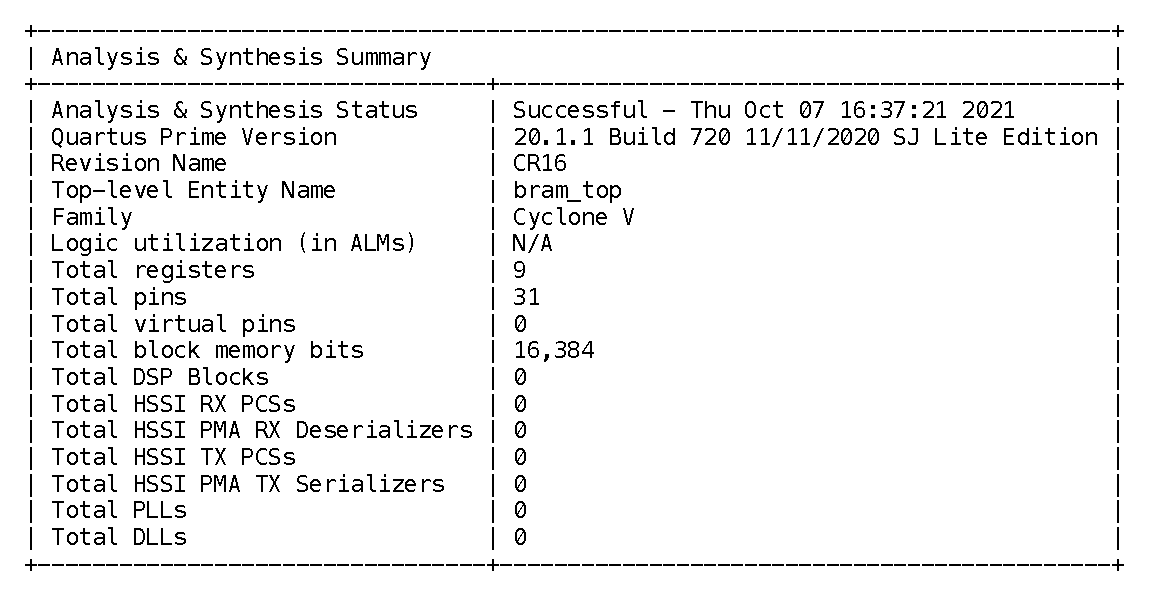
\includegraphics[scale=0.42]{resources/figures/summary_analysis_synthesis.pdf}
    \caption{High-level statistics of the Block RAM interface when synthesizing \emph{bram\_top.sv} as the top-level module.}
    \label{fig:summary_analysis_synthesis}
\end{figure}

\begin{figure}[htbp]
    \centering
    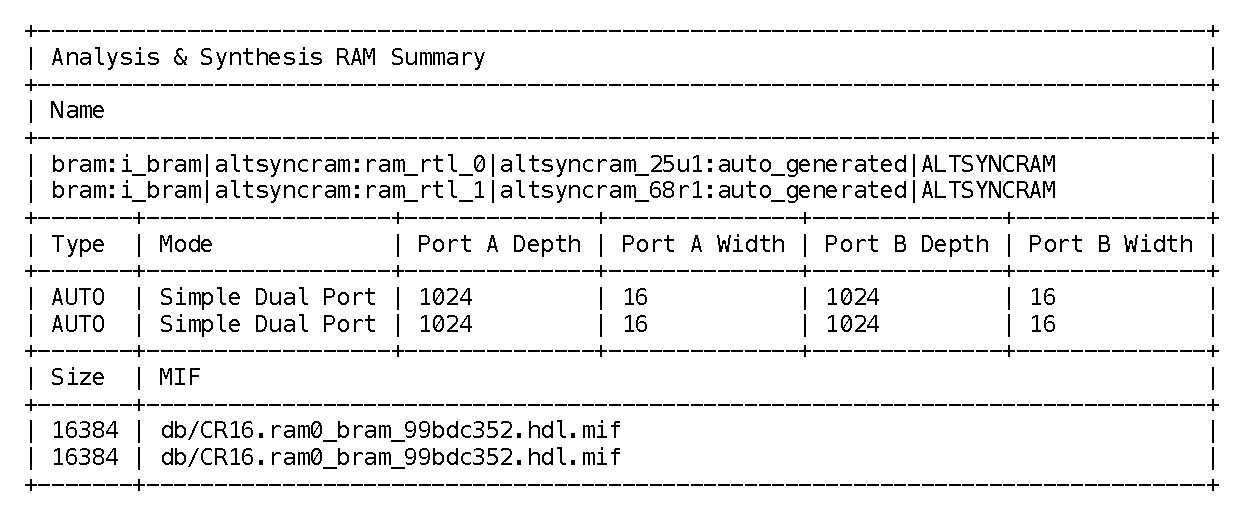
\includegraphics[scale=0.42]{resources/figures/summary_ram.pdf}
    \caption{Details of RAM usage for the Block RAM interface.}
    \label{fig:summary_ram}
\end{figure}

\begin{figure}[htbp]
    \centering
    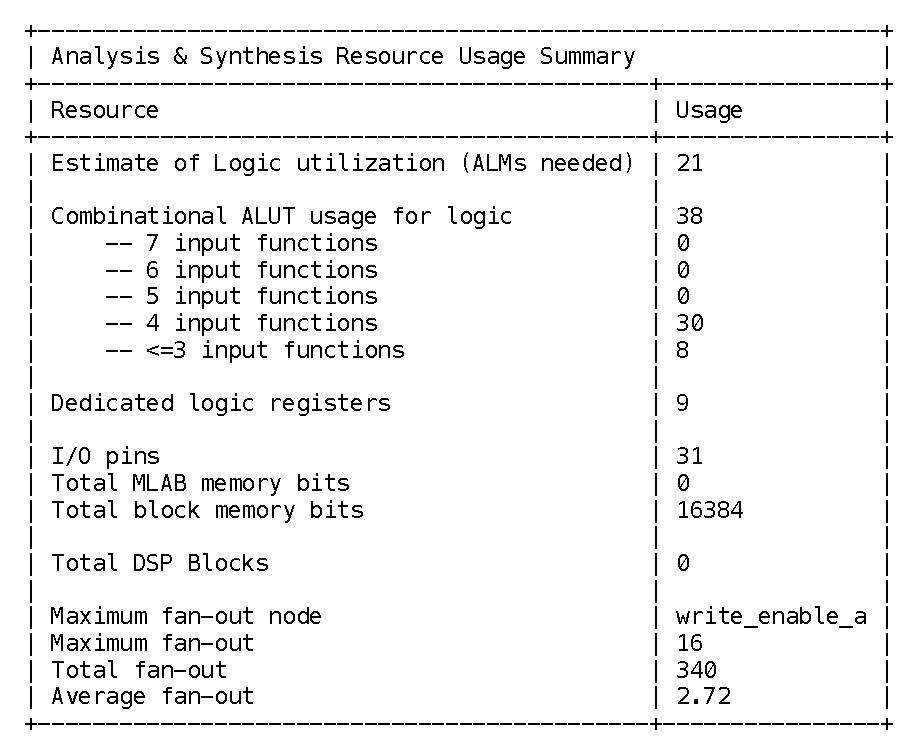
\includegraphics[scale=0.42]{resources/figures/summary_resource_usage.pdf}
    \caption{Details of resource usage for the Block RAM interface.}
    \label{fig:summary_resource_usage}
\end{figure}

\section{Conclusion}
The BRAM module is an essential component for efficient CPU functionality. By demonstrating correct functionality, we can be confident that our CPU will properly fetch instructions, write values, and navigate throughout the program based on coded control flow. We've shown correct operation in simulation and practice, so we are confident that the data will transfer properly. Although we were unable to run a proper instance of the Quartus Timing Analyzer, we are confident that there are no hold/setup time violations because the FSM we used to demonstrate on the FPGA was able to write and read on a single clock cycle. If this is an issue in the future, we can modify our FSM to handle setup, hold, and write-back. Based on the results we have seen so far, we are ready to begin integrating all of these elements together into one integrated datapath managed by a single CPU Finite State Machine.

\bibliographystyle{IEEEtran}
\bibliography{resources/bib/lab_3_ref.bib}
\end{document}
